\documentclass[12pt,a4paper,utf8x]{report}
\usepackage [frenchb]{babel}
\usepackage[pdftex]{graphicx}
%\usepackage{path}
% Pour pouvoir utiliser 
\usepackage{ucs}
\usepackage[utf8x]{inputenc}

\usepackage{url} % Pour avoir de belles url
\usepackage {geometry}

% Pour mettre du code source
\usepackage {listings}
% Pour pouvoir passer en paysage
\usepackage{lscape}

% Pour pouvoir faire plusieurs colonnes
\usepackage {multicol}
% POur crééer un index
\usepackage{makeidx}
\usepackage{color}

\usepackage{hyperref}
\usepackage{pdfpages}

\hypersetup{
    bookmarks=true,         % show bookmarks bar?
    unicode=false,          % non-Latin characters in Acrobat’s bookmarks
    pdftoolbar=true,        % show Acrobat’s toolbar?
    pdfmenubar=true,        % show Acrobat’s menu?
    pdffitwindow=false,     % window fit to page when opened
    pdfstartview={FitH},    % fits the width of the page to the window
    pdftitle={Documentation du flux},    % title
    pdfauthor={AUREGAN Pascal},     % author
    pdfsubject={Documentation du flux},   % subject of the document
    pdfcreator={AUREGAN Pascal},   % creator of the document
    pdfproducer={pdflatex}, % producer of the document
    pdfkeywords={keywords}, % list of keywords
    pdfnewwindow=true,      % links in new window
    colorlinks=true,       % false: boxed links; true: colored links
    linkcolor=Ror,          % color of internal links
    citecolor=green,        % color of links to bibliography
    filecolor=Ror,      % color of file links
    urlcolor=Ror           % color of external links
}
%fonte computer modern sans seriff

%\usepackage[T1]{fontenc}
%\usepackage{cmss}
%\newcommand\sfdefault{cmss}
\definecolor{Dark}{gray}{.2}
\definecolor{Medium}{gray}{.6}
\definecolor{Light}{gray}{.8}
\definecolor{Ror}{rgb}{0.65, 0.16, 0.16}

\newcommand*{\plogo}{
\includegraphics[clip=true, width=40mm, height=20mm]{./images/logo.jpg}}
%
\includegraphics[\textwidth,\textheight]{./images/logo.eps}
%pour une boite de couleur avec un texte de couleur
\newcommand{\boitecolor}[3]    {\colorbox{#1}{\textcolor{#2}{#3}}}

%\renewcommand{\paragraph}{\@startsection{paragraph}{4}{\z@}%
%            {-2.5ex\@plus -1ex \@minus -.25ex}%
%            {1.25ex \@plus .25ex}%
%            {\normalfont\normalsize\bfseries}}
            
%redefinition de la date
\date{	
	\normalsize{Lieu du stage\\
		Adresse du stage\\
		Ville du stage\\ 
		\vspace{5mm}	
		Directeur de recherche : M. DUPONT \\
		Rapporteur universitaire : Mme DUPUIS
	}
}

%Pour le titre joli
\newcommand*{\titleTH}{\begingroup% T&H Typography
	\protect\thispagestyle{empty}
	\begin{changemargin}{-2.5cm}{-1cm}
		\raggedleft
%		\vspace*{\baselineskip}
		{\Large Conservatoire National des Arts et Métiers}\\{\small Pascal AUREGAN}\\[0.167\textheight]

		{\bfseries Rapport de projet}\\[\baselineskip]
	%\end{changemargin}

%	\setlength{\textwidth}{208mm}
%	\begin{changemargin}{-2.5cm}{-1cm}
		\boitecolor{Ror}{white}{
			\makebox[208mm][r]{
				\Huge \textsf{NFE211}
		 }}\\[\baselineskip]
		%{\small illustrée}\par
		{\bfseries Test de chaine décisionnelle sur cas simple. }\\
		{\bfseries Base opérationnelle en fichier et PostgresSQL}\\
		{\bfseries ETL avec TALEND Data Integration,}\\
		{\bfseries Reporting avec SAS}\\
		\vfill

		{\Large \plogo}\par
		\vspace*{3\baselineskip}
	\end{changemargin}

	\pagebreak 
\endgroup}





\makeindex

% Pour les entetes de page

% \usepackage{fancyheadings}
%\pagestyle{fancy}
%\renewcommand{\sectionmark}[1]{\markboth{#1}{}} 
%\renewcommand{\subsectionmark}[1]{\markright{#1}} 

% Pour l'interligne de 1.5
\usepackage {setspace}
% Pour les marges de la page
\geometry{a4paper, top=2.5cm, bottom=3.5cm, left=2.5cm, right=1.5cm, marginparwidth=1.2cm}

\parskip=5pt %% distance entre § (paragraphe)
\sloppy %% respecter toujours la marge de droite 

% Pour les pénalités :
\interfootnotelinepenalty=150 %note de bas de page
\widowpenalty=150 %% veuves et orphelines
\clubpenalty=150 

%Pour la longueur de l'indentation des paragraphes
\setlength{\parindent}{15mm}



%%%% debut macro pour enlever le nom chapitre %%%%
\makeatletter
\def\@makechapterhead#1{%
  \vspace*{50\p@}%
  {\parindent \z@ \raggedright \normalfont
    \interlinepenalty\@M
    \ifnum \c@secnumdepth >\m@ne
        \Huge\bfseries \thechapter\quad
    \fi
    \Huge \bfseries #1\par\nobreak
    \vskip 40\p@
  }}

\def\@makeschapterhead#1{%
  \vspace*{50\p@}%
  {\parindent \z@ \raggedright
    \normalfont
    \interlinepenalty\@M
    \Huge \bfseries  #1\par\nobreak
    \vskip 40\p@
  }}
%
%\def\addcontentsline@toc#1#2#3{%
 % \addtocontents{#1}{\protect\thispagestyle{empty}}%
%   \addtocontents{#1}{\protect\contentsline{#2}{#3}{\thepage}}}
%\def\addcontentsline#1#2#3{%
 % \expandafter\@ifundefined{addcontentsline@#1}%
 % {\addtocontents{#1}{\protect\contentsline{#2}{#3}{\thepage}}}
 % {\csname addcontentsline@#1\endcsname{#1}{#2}{#3}}}

\makeatother
%%%% fin macro %%%%

%%%% debut macro %%%%
\newenvironment{changemargin}[2]{\begin{list}{}{%
\setlength{\topsep}{0pt}%
\setlength{\leftmargin}{0pt}%
\setlength{\rightmargin}{0pt}%
\setlength{\listparindent}{\parindent}%
\setlength{\itemindent}{\parindent}%
\setlength{\parsep}{0pt plus 1pt}%
\addtolength{\leftmargin}{#1}%
\addtolength{\rightmargin}{#2}%
}\item }{\end{list}}
%%%% fin macro %%%%

%Couverture 

\title
{
	\normalsize{DESS Xxxxx xxxx xxxxx\\
	Université de Xxxx Xxxxxx\\
	2004-2005}\\
	\vspace{15mm}
	\Huge{Titre du rapport de stage}
}
\author{Nom Auteur\\
	\vspace{45mm}
}



\renewcommand{\familydefault}{\sfdefault}
\begin{document}

%\setlength{\hoffset}{-1.5cm}
%\addtolength{\textwidth}{1cm}

\titleTH




%\setlength{\hoffset}{-1.5cm}


	\tableofcontents
	\clearpage

	% Pour avoir un interligne de 1,5
	\begin{onehalfspace}

		\chapter{Introduction}

Le but de se projet est de mettre en place une chaine décisionnelle. L'objectif de ce projet n'étant pas de pousser dans ses retranchements les outils de la chaine décisionnelle, il a été décidé de créer de toute pièce un jeu de données. Le thème de ce jeu de données est l'achat de BD comme dans le cours. 
La base opérationnelle décrit les factures d'un ensemble librairies en France dont les clients sont connus.
La chaine décisionnelle doit être en mesure de répondre in fine à la question: analyser les ventes de BD en France en fonction des clients, du lieu et date d'achat.
La couche opérationnelle est assurée par une base de données de fichier csv et une base de données PostgresSQL. 

Pour la couche ETL, il a été choisi TALEND Data Integration. 

La couche reporting étudiée lors de ce projet est assurée par SAS Studio Version Etudiante.


\includegraphics[clip=true, width=120mm, height=80mm]{images/chaine.png} 
\label{chaine}



\clearpage


		%\chapter{Flux de données: flux{\_}vls (PAU)}
\chapter{Spécifications}
\section{Spécification fonctionnelle}
\subsection{Présentation}
Nous nommons flux{\_}vls l'ensemble des applications gérant les différents processus allant de l'obtention des données jusqu'à l'agrégation des données stockées. Les données sont les valeurs liquidatives datées des fonds trouvés. Nous appelons fonds un portefeuille de titres géré par un professionnel et proposé par un établissement financier ou une banque. Flux{\_}vls est donc composé d'un processus d'obtention des données, un processus d'intégration des données et un processus d'agrégation et de préparation des données. Il existe aussi un processus chargé de la maintenance de la base ou du moins ce qui peut être traité de manière automatique.
\subsection{Processus d'obtention des données}
Nous appelons donnée le tuple $\lbrace ISIN\protect\footnote{International Securities Identification Number}, devise, VL\protect\footnote{Valeur Liquidative}, date\ de\ la\ valorisation \rbrace$. L'isin est un code à 12 caractères permettant d'identifier les valeurs de manière internationale.\\
Les données sont obtenues par robot web.\\
Chaque soir le processus lance un robot web par fournisseur agrégé \textit{(voir la liste des fournisseurs agrégés \ref{fournisseurs} page~\pageref{fournisseurs})}.\\
Le robot web se connecte au site web du fournisseur.\\
Le robot web met les données au format {\og}$ISIN;DEV;VL(ex:10.00);jj/mm/aaaa${\fg}  dans un fichier textué.\\
Le robot web crée donc un fichier par fournisseur.\\
Un robot web supplémentaire est destiné à obtenir les taux de conversion DEV$\rightarrow$EUR avec le format {\og}$DEV;jj/mm/aaaa;taux(ex:10.00)${\fg}  de manière à ce qu'on ait $1 EUR = taux \times DEV$.

\subsection{Processus d'intégration des données et base de données associée}
Les fichiers créés par le processus d'obtention des données sont ouverts un par un et leur contenu est stocké dans une base de données appellée flux{\_}vls.
Le processus vérifie que les données ne sont pas trop absurdes.
On entend par absurde le fait qu'un tuple candidat à l'insertion ne vérifie pas le bon format ou que la date de la valeur soit supérieure à la date du jour.

\subsection{Processus d'agrégation et de préparation des données, base de données associée et calcul des taux d'évolution}
L'ensemble des données stockées dans flux{\_}vls est par ce processus restreint à l'ensemble des données qui concernent CYRUS CONSEIL (soit $\approx$ 1 000 fonds). Les données qui concernent CYRUS CONSEIL sont les valeurs des supports dont le montant souscrit est supérieur à 0 et possédant un ISIN. La discrimination se fait à partir de la base du système d'informations ajourd'hui appelée BDD8DEFSQL.\\ 
La base de données contenant les données restreintes sera appelée flux{\_}vls{\_}eur. flux{\_}vls{\_}eur est différente de la base contenant la totalité des données. Ainsi, si BDD8DEFSQL comporte des informations erronnées, la contamination ne se propage que dans flux{\_}vls{\_}eur. flux{\_} est ainsi protégée de toute contamination externe.\\
Les calculs des taux d'évolution s'effectuent à partir de flux{\_}vls{\_}eur. De cette manière on ne fait des calculs que pour les fonds dont on a besoin. Cela permet de diminuer le temps de calcul qui est déjà très long (5 heures). Le résultat des calculs est stocké dans une table prête à servir facilement.

\subsection{Processus de maintenance de la base}
Il existe un processus lancé quotidiennement qui sauvegarde et archive flux{\_}vls et flux{\_}vls{\_}eur. Il est normalement fait un vacuum. Il faudrait ajouter à cela un réindexage total lancé de manière bimensuelle. Il existe un outil pour créer une table de performances arrêtées à une date.
\clearpage
\section{Rôle et identification des différents fichiers}
\subsection{Présentation}
Nous allons dans cette section décire les différents fichiers intervenant dans le flux de valeurs liquidatives. Pour les bases de données on donnera simplement le diagramme.
\subsection{Bases de données}
\subsubsection{Base de données flux{\_}vls}
	\begin{changemargin}{-2.5cm}{-1cm}
		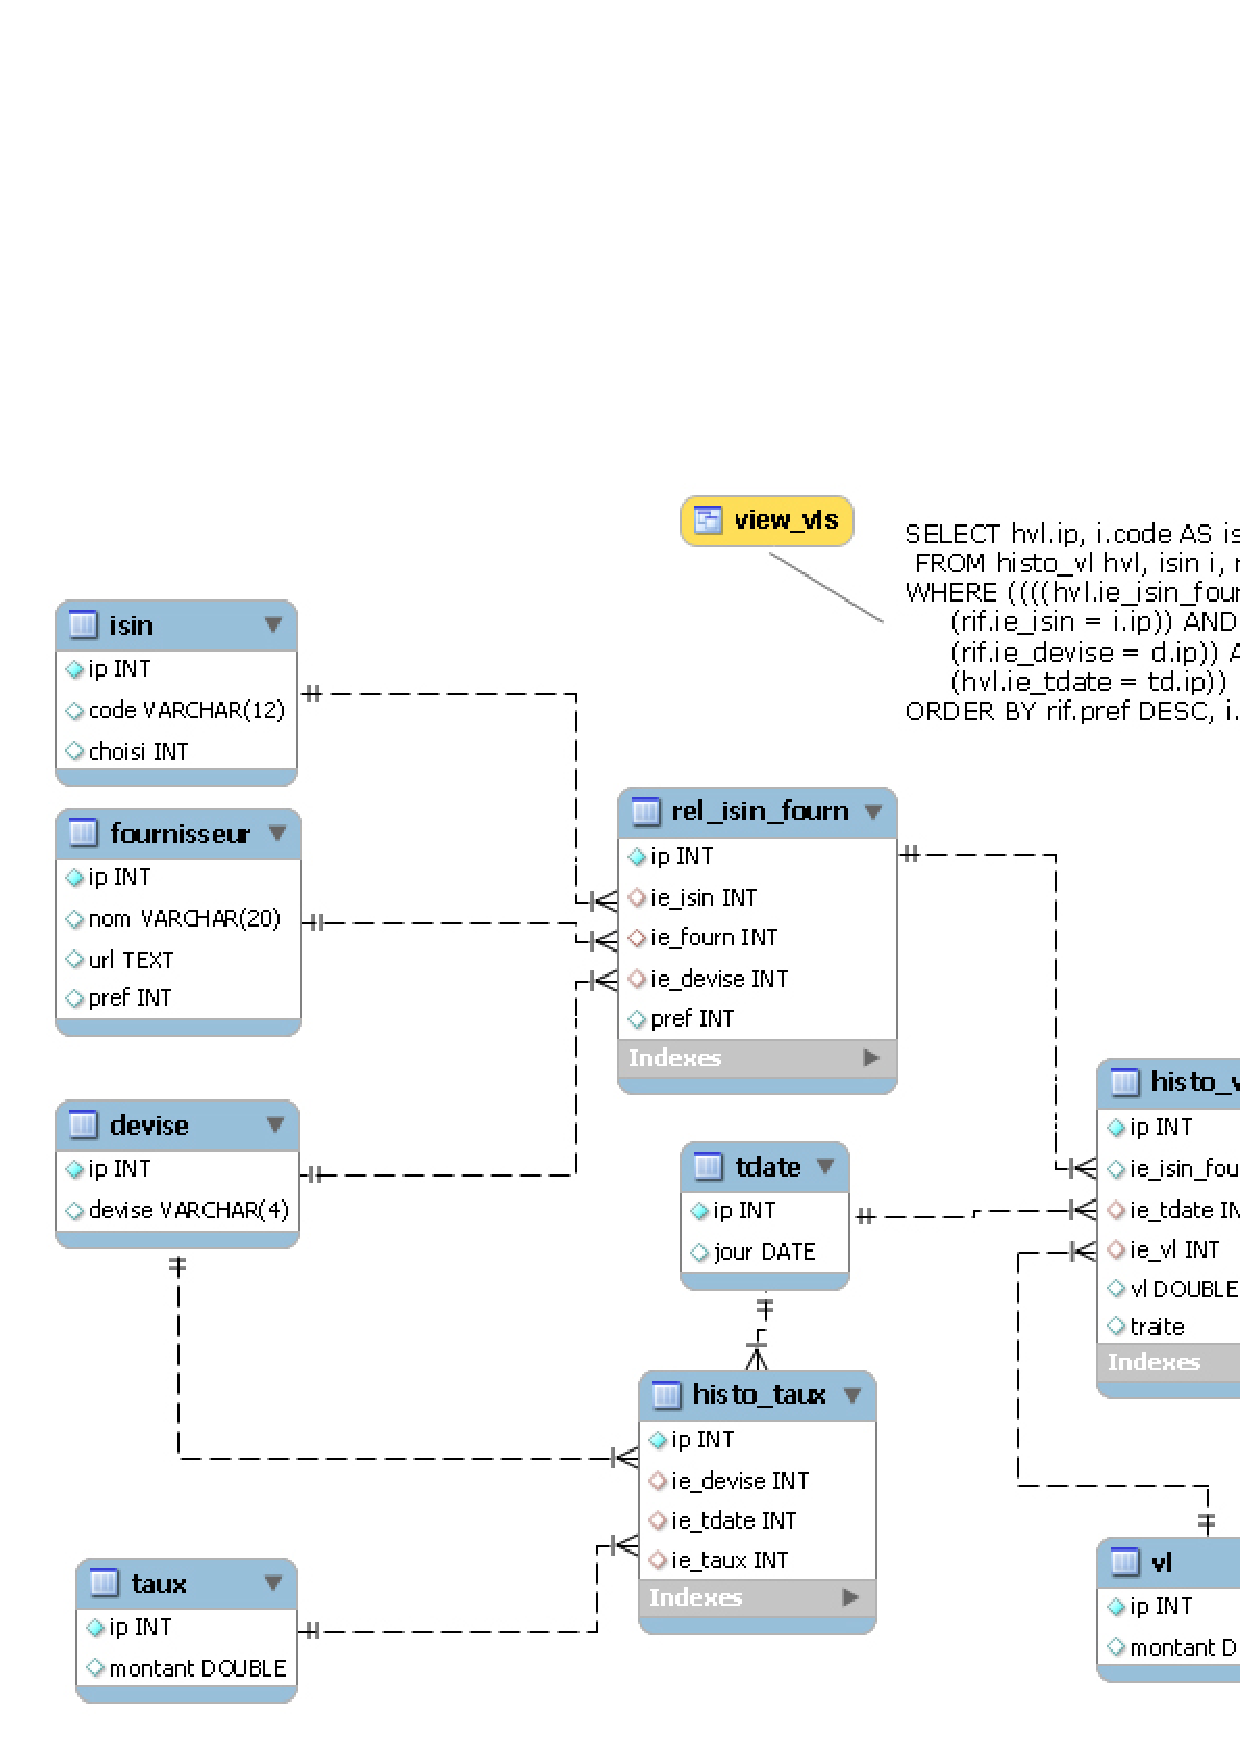
\includegraphics[scale=0.6]{images/flux_vls_map.png} 
	\end{changemargin}
	\clearpage
\subsubsection{Base de données flux{\_}vls{\_}eur}
	\begin{changemargin}{-2.5cm}{-1cm}
		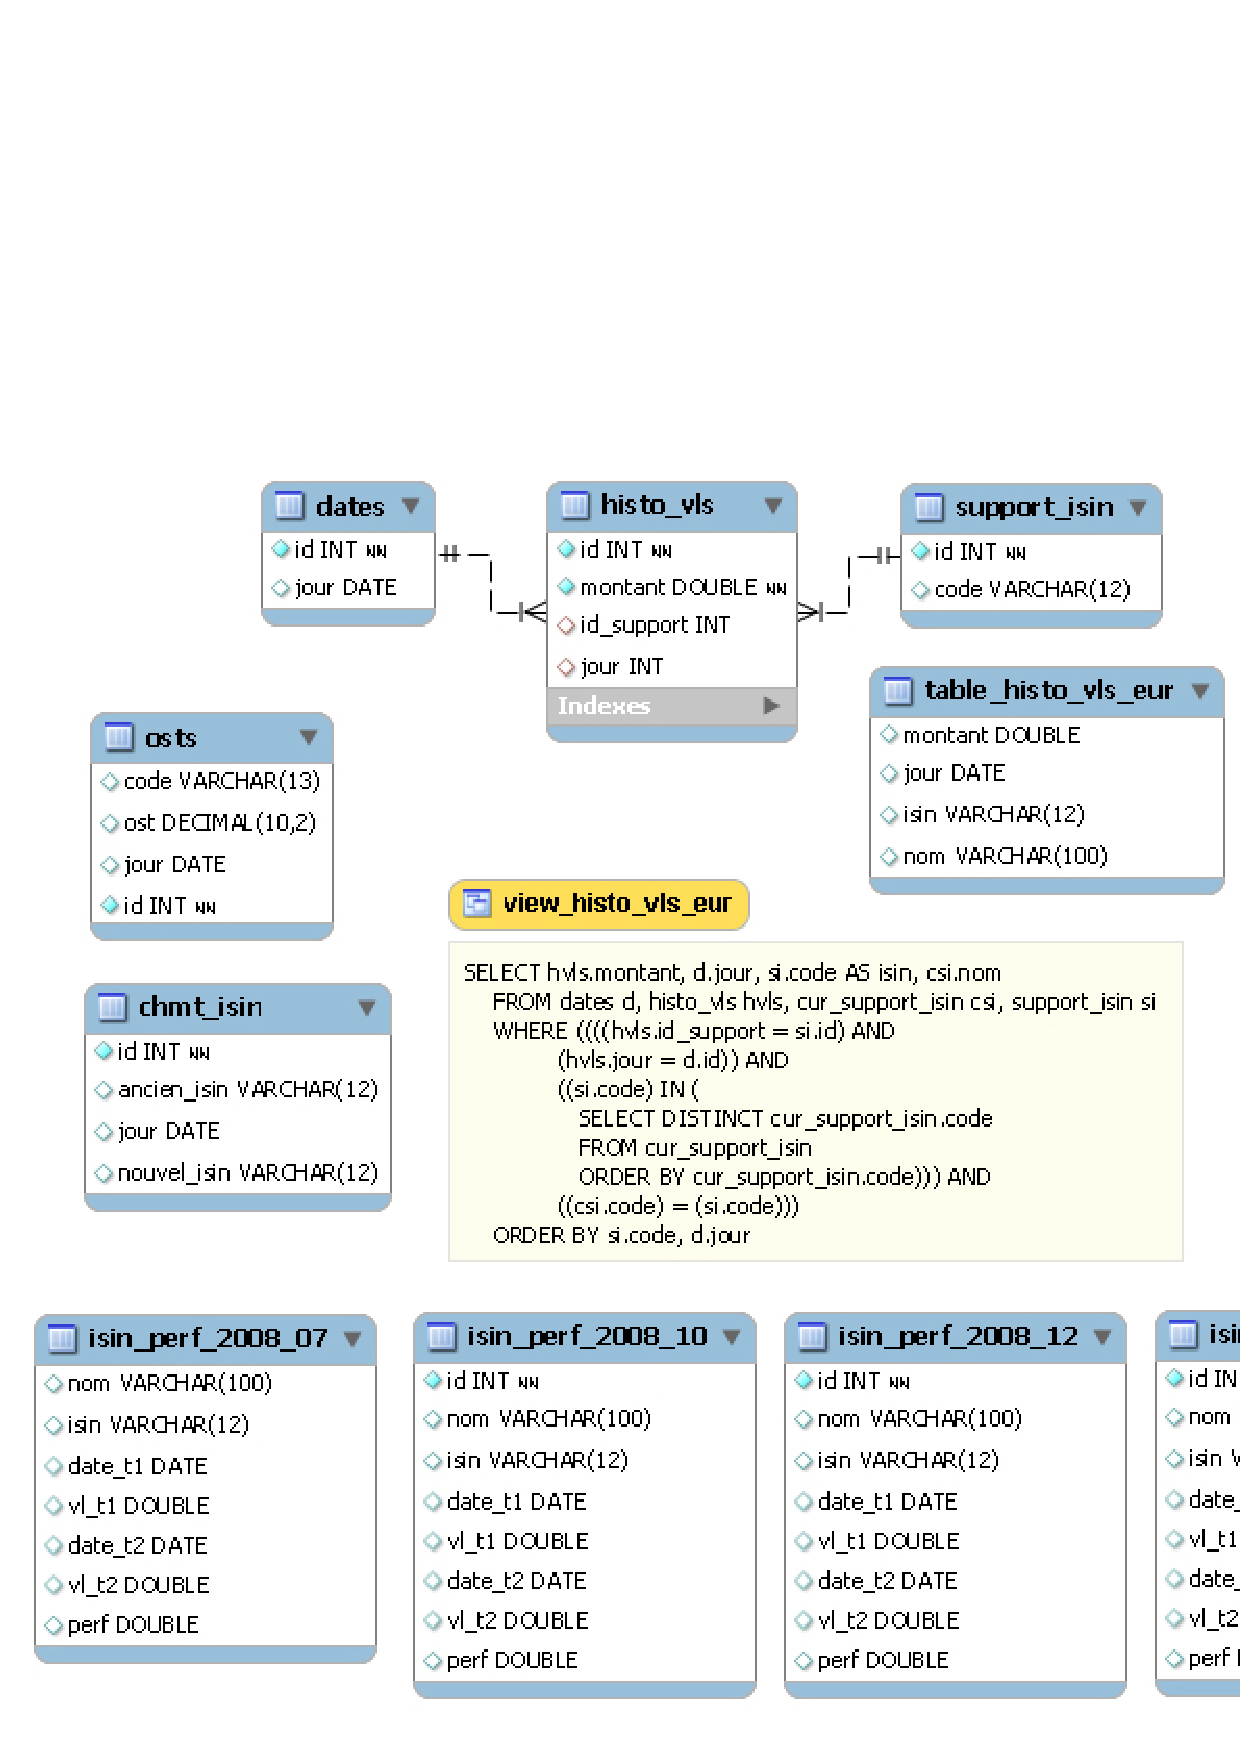
\includegraphics[scale=0.6]{images/flux_vls_eur_map.png} 
	\end{changemargin}	
\subsubsection{Programmes}
\paragraph{/home/postgres/db/script/do{\_}back{\_}up.sh} Lancé par le cron de postgres quotidiennement.\\
Ici, {\$}TODAY représente la date du jour. {\$}TODAY est déterminé avec la commande bash :
\lstset{language=bash}
\begin{lstlisting}
 `date +"{\%}Y{\%}m{\%}d-{\%}H"`
\end{lstlisting}
Ce que fait le fichier : 
\begin{enumerate}
\item Crée un répertoire /home/postgres/db/backup/{\$}TODAY,
\item Sauvegarde la base de données flux{\_}vls dans le fichier flux{\_}vls{\$}TODAY.sql via pg{\_}dump,
\item Sauvegarde la base de données flux{\_}vls{\_}eur dans le fichier flux{\_}vls{\_}eur{\$}TODAY.sql via pg{\_}dump,
\item Le répertoire {\$}TODAY est {\og}taré{\fg}  et {\og}gzipé{\fg}  via tar -cvzf,
\item Le serveur de bases de données est redémarré.
\end{enumerate}
\paragraph{/home/malko/flux{\_}vls/outils/create{\_}isin{\_}perf{\_}arretee.rb} \label{arret-perf}Lancé manuellement avant chaque génération des états de compte.\\
Ce programme crée une table de la forme : isin{\_}perf{\_}yyyy{\_}mm avec yyyy{\_}mm l'année (2009 par exemple) et le mois (07 par exemple).\\
Ce programme s'utilise comme suit :\\
La table de performances arrêtées se crée le 02 ou le 03 du mois pour avoir les données du 1\up{er} du mois.
\begin{enumerate}
\item Se connecter sur la machine du flux (actuellement prodserver : 192.168.0.78),
\item Aller dans \path{/home/malko/flux_vls/outils},
\item ruby create{\_}isin{\_}perf{\_}arretee.rb,\\
\includegraphics[clip=true, width=335px, height=225px]{./images/creation.jpg}\\
\item Choisir 3 dans la plupart des cas,
\item Suivre ce qui est indiqué.
\end{enumerate}
	\clearpage
\subsection{Processus d'obtention des données}
Dans la suite de ce document nous appelons \path{#} \path{/home/malko/flux_vls/}.\\
\subsubsection{Programmes}
\paragraph{{\#}/imports/import{\_}vl.sh} Lancé par le cron.
\begin{itemize}
\item Création du fichier \path{#/imports/a_import.py} par le script \path{#/imports/creation_fichier_import.py}.\\
Du code python est créé pour gérer chaque robot.\\
Exemple du code créé dans le fichier a{\_}import.py (ici gestion du robot cardif): \\
\lstset{language=python, keywordstyle=\color{Ror}}
\lstset{frame=shadowbox, rulesepcolor=\color{Ror}}
\begin{lstlisting}
import os
import datetime
import fournisseurs.import_cardif
global repertoire_fichiers
repertoire_fichiers = '/home/malko/flux_vls/fichiers/'
def file_exists(fichier):
    try:
        file(fichier)
        return True
    except:
        return False
if file_exists('log/imports.log'):
    os.remove('log/imports.log')
file_log = open('log/imports.log', 'a')
try:
    print "debut " + "cardif"
    fournisseurs.import_cardif.import_cardif()
except Exception, e:
    print "!!!!!!!!!!!!!!cardif a plante"
    print e
    fichier = '/home/malko/flux_vls/imports/' +
	'fournisseurs/import_cardif.py\n'
    file_log.write(fichier)
file_log.close()
\end{lstlisting}
\item Lancement du script \path{#/imports/a_import.py}.\\
	L'historique des évènements s'enregistre dans le fichier \path{#/imports/log/imports.log}.\\
	Ce script lance les robots.
\item Lancement de \path{#/import_ds_bdd.rb}
\end{itemize}
\paragraph{robots}
\label{robots}
Les robots sont dans le répertoire \path{#/imports/fournisseurs/}. Un robot a comme nom de fichier import{\_}fournisseur.py où fournisseur est le nom du fournisseur. Un robot peut avoir aussi un fichier import{\_}fournisseur.rb mais il faut impérativement qu'il y ait un fichier import{\_}fournisseur.py. Un fichier python contient obligatoirement une méthode comme : 
\lstset{language=python, keywordstyle=\color{Ror}}
\lstset{frame=shadowbox, rulesepcolor=\color{Ror}}
\begin{lstlisting}
def import_fournisseur():
	#code du robot ou 
	#appel du robot ruby import_fournisseur.rb
\end{lstlisting}
Les robots utilisent les fichiers \path{#/imports/fournisseurs/support.py} pour les robots entièrement en python et \path{#/imports/fournisseurs/support.rb} pour les robots mi--python/mi--ruby. Ces fichiers contiennent les classes $Support(isin, devise, vl, date)$.\\
Le robot morningstar est particulier : il se trouve dans le répertoire \path{#/imports/fournisseurs/robot_morningstar} et est lancé séparément par son propre cron.
\paragraph{{\#}/imports/manage{\_}robot.sh}
Ce que fait ce script :
\begin{itemize}
	\item Efface les fichiers python et ruby du fournisseur.
		Pour créer les fichiers python et ruby il faut avoir enlevé du répertoire \path{#/imports/fournisseurs/} les fichiers \path{import_fournisseur.py} et \path{import_fournisseur.rb} car on veut être sûr de ne pas supprimer un fichier par inadvertance.
	\item Crée les fichiers python et ruby nécessaires au robot fournisseur à partir des modèles \path{#/imports/fournisseurs/modele/import_modele.[py|rb]}.
	\item Ouvre les fichiers python et ruby du robot fournisseur.	
\end{itemize}
\includegraphics[clip=true, width=500px, height=150px]{./images/robot.jpg}\\
\paragraph{{\#}/fichiers/import{\_}fournisseur.txt $\vert$ taux{\_}ecb.txt}
\label{fichiers-flux}
Ce sont les fichiers produits par les robots.
Ces fichiers sont importés puis archivés.\\
Exemple de fichier import{\_}fournisseur.txt
\lstset{language=python, keywordstyle=\color{Ror}}
\lstset{frame=shadowbox, rulesepcolor=\color{Ror}}
\begin{lstlisting}
FR0010129114;63.07;EUR;28/07/2009
\end{lstlisting}
Exemple de fichier taux{\_}ecb.txt :
\lstset{language=python, keywordstyle=\color{Ror}}
\lstset{frame=shadowbox, rulesepcolor=\color{Ror}}
\begin{lstlisting}
LTL;30/07/2009;3.4528
\end{lstlisting}

\subsubsection{Fichiers logs}
\paragraph{{\#}/imports/log/imports.log}
La partie de ce fichier qui nous intéresse ici est la partie liée aux téléchargements des robots. Lorsque un robot plante, une première indication est écrite.\\
Exemple d'une ligne de log pour ecofi :
\lstset{language=python, keywordstyle=\color{Ror}}
\lstset{frame=shadowbox, rulesepcolor=\color{Ror}}
\begin{lstlisting}
debut ecofi
"ECOFI:::FR0010706549::: non trouve"
\end{lstlisting}
\paragraph{{\#}/imports/log/log{\_}sp.log}
On trouve dans ce fichier les liens morningstar visités.
\subsection{Processus d'intégration des données}
\subsubsection{Programmes}
\paragraph{{\#}/import{\_}ds{\_}bdd.rb}
Ce programme importe les fichiers présents dans \path{#/fichiers/}. Les taux taux{\_}ecb.txt sont importés en premier. Les fichiers import{\_}fournisseur.txt sont importés ensuite.
\paragraph{{\#}/imports/backup{\_}import{\_}files{\_}bdd.rb}
Ce programme archive dans \path{#/fichiers/backup} les fichiers présents dans \path{#/fichiers/}. Les archives créés à partir de {\og}tar -cvzf{\fg}  se nomment sous la forme yyyymmdd-hh.tgz où yyyy, mm, dd, hh représentent respectivement l'année (ex : 2009), le mois (ex : 05 pour le mois de Mai), le jour (ex : 31) et l'heure (ex : 02 pour 2 heures du matin).
\subsubsection{Fichiers logs}
\paragraph{{\#}/imports/log/imports.log}
\subparagraph{{\#}/import{\_}ds{\_}bdd.rb}
Exemple pour l'import d'ecofi:
\lstset{language=python, keywordstyle=\color{Ror}}
\lstset{frame=shadowbox, rulesepcolor=\color{Ror}}
\begin{lstlisting}
::2009-08-01 08:59 => updating database...
"00:48 => debut ecofi"
"00:50 => fin ecofi"
::2009-08-01 08:59 => database updated
\end{lstlisting}
\subparagraph{{\#}/imports/backup{\_}import{\_}files{\_}bdd.rb}
Exemple de sauvegarde :
\lstset{language=python, keywordstyle=\color{Ror}}
\lstset{frame=shadowbox, rulesepcolor=\color{Ror}}
\begin{lstlisting}
::2009-08-01 02:43 => changing directory to 
	/home/malko/flux_vls/imports/ successed
::2009-08-01 02:43 => creating 20090801-02 directory ...
::2009-08-01 02:43 => moving files to 20090801-02 directory...
20090801-02/
20090801-02/import_ecofi.txt
::2009-08-01 02:43 => directory saved
\end{lstlisting}
\subsection{Processus d'agrégation, de préparation des données et calcul des taux d'évolution}
\subsubsection{Programmes}

\paragraph{{\#}/imports/import{\_}mssql/import{\_}mssql.sh} (Lancé par le cron) Lance successivement \path{#/imports/import_mssql/import_mssql.rb}, \path{#/imports/import_mssql/comp_perf.rb}, \path{#/mail/mail.py}

\paragraph{Sur ServeurBDD :}

\subparagraph{C:{\textbackslash}workspace{\textbackslash}python{\textbackslash}supports{\_}utilises{\textbackslash}script{\textbackslash}do{\_}maj{\_}supports.bat\\} Lancé quotidiennement à 22h30 par le gestionnaire de t\^aches planifiées de $Windows^{\textregistered}$. Lance le script C:{\textbackslash}workspace{\textbackslash}python{\textbackslash}supports{\_}utilises{\textbackslash}script{\textbackslash}supports{\_}utilises.py

\subparagraph{C:{\textbackslash}workspace{\textbackslash}python{\textbackslash}supports{\_}utilises{\textbackslash}script{\textbackslash}supports{\_}utilises.py\\}Crée le fichier \url{http://192.168.0.1:81/supports/supports.xml} qui se trouve dans C:{\textbackslash}workspace{\textbackslash}python{\textbackslash}supports{\_}utilises{\textbackslash}rendu à partir de la base de données {\og}BDD8DEFSQL{\fg} . Le script se connecte à la base {\og}BDD8DEFSQL{\fg}  et serialise en xml les données de la vue {\og}used{\_}supports{\fg} . La vue {\og}used{\_}supports{\fg}  est le résultat de la requ\^ete suivante : 
\lstset{language=sql, keywordstyle=\color{Ror}}
\lstset{frame=shadowbox, rulesepcolor=\color{Ror}}
\begin{lstlisting}
SELECT DISTINCT TOP (100) PERCENT dbo.supports.ISIN,
dbo.supports.id_support, dbo.supports.nom, l.libelle
FROM         dbo.libelles AS l INNER JOIN
                     dbo.supports LEFT OUTER JOIN
                     dbo.contrat_support ON dbo.supports.id_support =
dbo.contrat_support.id_support ON l.id = dbo.supports.flux_label
WHERE     (dbo.supports.ISIN IS NOT NULL)
GROUP BY dbo.contrat_support.id_support, dbo.supports.ISIN,
dbo.supports.id_support, dbo.supports.nom, l.libelle
HAVING      (SUM(dbo.contrat_support.montant) > 0) OR
                     (l.libelle NOT LIKE 'BASIQUE')
ORDER BY dbo.supports.id_support
\end{lstlisting}

\subparagraph{\textbf{http://192.168.0.1:81/supports/supports.xml}\\}
Voici un exemple de ce fichier :\\
\lstset{language=xml, keywordstyle=\color{Ror}}
\lstset{frame=shadowbox, rulesepcolor=\color{Ror}}
\begin{lstlisting}
<?xml version="1.0" encoding="ISO-8859-1"?>
<supports>
	<support 
		isin="FR0010551424" 
		id_support="5711" 
		nom="DARWIN DIVERSIFIE 60-80 1/1.000" 
		flux_label="BASIQUE"
	/>
</supports>
\end{lstlisting}
flux{\_}label prend ses valeurs dans $\lbrace "BASIQUE", "PERF", "PERF{\_}ET{\_}MORN"\rbrace $
\begin{itemize}
\item $"BASIQUE"$ désigne un fonds dont le montant total agrégé est strictement positif.
\item $"PERF"$ oblige le flux à récupérer la vl du fonds. Il faut utiliser ce label lorsque le fonds est déjà dans flux{\_}vls mais que le montant total agrégé est nul (et si on a besoin de la performance du fonds).
\item $"PERF{\_}ET{\_}MORN"$ oblige le flux à récupérer la vl du fonds par le robot morningstar. Il faut utiliser ce label lorsque le fonds n'est pas dans flux{\_}vls mais que le montant total agrégé est nul (et si on a besoin de la performance du fonds).
\end{itemize}
Il faut bien évidemment penser à mettre à jour les labels des supports pour ne pas faire de requ\^etes inutiles.

\paragraph{{\#}/outils/chmt{\_}isin/chmt{\_}isin.sh}\label{chmt-isin} Lancé par le cron. Met à jour les données relatives aux changements d'isin et aux divisions de valeurs liquidatives des fonds.\\
Ce que fait ce fichier : 
\begin{itemize}
\item Se connecte à la base {\og}outil{\_}produit{\fg}  sur le serveur 192.168.0.74,
\item Sérialize dans \path{#/outils/chmt_isin/chmt_isin.txt} la table {\og}changer{\_}isin{\fg} ,
\item Remplit la table {\og}chmt{\_}isin{\fg}  de la base les données {\og}flux{\_}vls{\_}eur{\fg}  à partir des données de \path{#/outils/chmt_isin/chmt_isin.txt},
\item Sérialize dans \path{#/outils/chmt_isin/osts.txt} la table {\og} splits{\fg},
\item Remplit la table {\og}osts{\fg}  de la base de données {\og}flux{\_}vls{\_}eur{\fg}  à partir des données de \path{#/outils/chmt_isin/osts.txt}.
\end{itemize}

\paragraph{{\#}/imports/import{\_}mssql/import{\_}mssql.rb} Se sert du fichier \url{http://192.168.0.1:81/supports/supports.xml} pour conna\^itre la liste des fonds dont la performance doit \^etre calculée. \\
Ce que fait ce fichier :
\begin{itemize}
\item vide puis remplit la table  {\og}table{\_}vls{\fg}  de {\og}flux{\_}vls{\fg}  à partir de la vue {\og}view{\_}vls{\fg},
\item remplit la table  {\og}cur{\_}support{\_}isin{\fg}  à partir de \url{http://192.168.0.1:81/supports/supports.xml},
\item fait passer toutes les vls connues de ces fonds dans la base de données  {\og}flux{\_}vls{\_}eur{\fg},
\item vide puis remplit la table  {\og}table{\_}histo{\_}vls{\_}eur{\fg}  de la base {\og}flux{\_}vls{\_}eur{\fg}  à partir de la vue  {\og}view{\_}histo{\_}vls{\_}eur{\fg}.
\end{itemize}

\paragraph{{\#}/imports/import{\_}mssql/comp{\_}perf.rb}
Calcule les performances pour les fonds de la table {\og}cur{\_}support{\_}isin{\fg}  qui sont présents dans la base de données flux{\_}vls. Se sert de la table {\og} osts{\fg} et {\og} chmt{\_}isin{\fg}. La performance des fonds au jour $j$ de l'année $n$ est calculée entre le 31 Décembre de l'année $n-1$ --- ou la date de création du fonds si le fonds est créé l'année durant --- et la dernière date de valorisation connue. 

\paragraph{{\#}/mail/mail.py}
Récupère tous les logs de \path{#/imports/log} et de \path{#/imports/import_mssql/log} et les envoie par mail aux destinataires choisis.

\subsubsection{Fichiers logs}
\paragraph{{\#}/imports/import{\_}mssql/log/log{\_}cron.log}
Fichier log du cron pour le \path{#/imports/import_mssql/import_mssql.sh}.\\Généralement rien ne se passe dans ce fichier.
\paragraph{{\#}/imports/import{\_}mssql/log/log{\_}mssql.log}
Fichier log de ce qui est fait dans {\#}/imports/import{\_}mssql/import{\_}mssql.rb.\\
Il y a très rarement des problèmes.
\paragraph{{\#}/imports/import{\_}mssql/log/log{\_}comp.log}
Fichier log de ce qui est fait dans {\#}/imports/import{\_}mssql/comp{\_}perf.rb.
Il y a très rarement des problèmes.
\paragraph{{\#}/imports/import{\_}mssql/log/log{\_}mail.log}
Fichier log de l'envoi des mails quotidiens de compte--rendu.
Il y a très rarement des problèmes.

\chapter{Maintenance de l'application}
Cette partie sera présentée sous forme de F.A.Q (Frequently Asked Questions).
\section{Comment arrêter la situation à une date choisie}
 voir \ref{arret-perf}
\section{Comment ajouter une situation}
voir \ref{fichiers-flux}
Créer le fichier comme indiqué et importer le fichier avec \path{#/imports/backup_import_files_bdd.rb}. Si on a besoin de la performance avant le lendemain on lance \path{#/imports/import_mssql/import_mssql.sh} sinon on laisse faire le flux et le lendemain les performances seront à jour.

\section{Comment ajouter ou réparer un robot?}
Pour ajouter un robot : 
\begin{itemize}
\item Vérifier que l'on a bien le tuple $\lbrace ISIN\protect\footnote{International Securities Identification Number}, devise, VL\protect\footnote{Valeur Liquidative}, date\ de\ la\ valorisation \rbrace$ sur le site. Si on n'a pas exactement ce tuple, il ne faut pas faire de robot. La date de valorisation doit \^etre inscrite sur le site : elle ne doit pas \^etre d\'eduite \`a partir de la date du jour.
\item Penser \`a injecter les valeurs des fonds au 31/12 pour que la performance calculée soit juste.
\item Implémenter le robot (voir \ref{robots})
\end{itemize}

Pour tester puis réparer le cas échéant le robot :
\lstset{language=bash, keywordstyle=\color{Ror}}
\lstset{frame=shadowbox, rulesepcolor=\color{Ror}}
\begin{lstlisting}
cd "#/imports";
#fournisseur = nom du founisseur
#fournisseurs = repertoire fournisseurs 
#et non pas nom du fournisseur avec un s
python test_fourn.py fournisseurs/import_fournisseur.py;
\end{lstlisting}
Le flux lancera automatiquement le robot le lendemain.

\paragraph{Suggestions : } il faudrait finir le robot acropole.
\section{Comment vérifier les résultats?}
Regarder le mail envoyé chaque jour et réparer ce qui ne va pas.\\
Si lcf ne fonctionne pas, c'est certainement qu'il faut relancer quelques firefox -jssh : en lancer un dans un terminal puis quelques autres à partir d'un autre terminal.\\
Le site des caisses d'épargnes ne fonctionne plus (ce) : il manque des données. Lodh ne fonctionne plus non plus ainsi que Crédit suisse et suravenir. Il faut aller régulièrement sur leur site respectif pour voir si on ne peut pas réintégrer un robot.\\
Un fonds de Cardif n'est pas trouvé. Pour euro tunnel dans la partie calcul de performance, il s'agit d'un problème de l'amf. Il faut savoir aussi que l'amf et afer (et pourquoi pas d'autres?) nous donne parfois des valeurs liquidatives valides dans plusieurs années.\\
Si la machine plante au milieu de la nuit, regarder dans \path{#/fichiers/} si les fichiers d'imports sont présents. Si les fichiers sont pr\'esents, taper la commande suivante en se pla\c cant dans \path{#} :\\
\lstset{language=bash, keywordstyle=\color{Ror}}
\lstset{frame=shadowbox, rulesepcolor=\color{Ror}}
\begin{lstlisting}
ruby import_ds_bdd.rb
\end{lstlisting}
Le calcul des performances peut attendre le lendemain.
\section{Comment traiter les OST/Changement ISIN?}
voir \ref{chmt-isin}

\section{Comment s'occuper du flux?}
Il faut \^etre convaincu qu'on est sûr de rien. Par conséquent, il faut tout vérifier avant de faire quoique ce soit m\^eme si on pense savoir. Si il nous est rapporté qu'il y a une erreur, on vérifie toujours et on ne rentre pas des valeurs pour faire plaisir à un tel ou à un autre. Si on pense qu'il n'y a pas d'erreur, on vérifie quand m\^eme : on a parfois des surprises.

\section{A quelle heure peut on vérifier les données?}
Le mail de logs arrive généralement vers 12h50. Si l'heure d'arrivée du mail s'écarte trop de cette heure, c'est qu'il doit y avoir un problème. Il faut effectuer les modifications jusqu'\`a 18h environ. Il ne faut pas redémarrer la machine avant 17h30 car le robot Morningstar tourne.
toto
\clearpage


		
\chapter{TALEND Open Studio for Data Integration 5.6}

\section{Création du modèle OLAP}
\subsection{Question à répondre}
Analyse des ventes de bande dessinées d'une enseigne de librairie possédant plusieurs boutiques dans plusieurs villes.

\subsection{Modèle ROLAP}

L'implémentation ROLAP a été choisie par rapport au modèle MOLAP car même si la quantité de données était petite, il m'a semblé important d'étudier ce modèle qui paraît être très utilisé. Ne voyant rien justifier un modèle en flocon permettant de gagner de l'espace de stockage, j'ai utilisé un modèle en étoile.
La table de faits est la table vente. Les dimentsions sont le temps, la boutique(lieu d'achat), le client, et le livre. L'étoile est de type transaction.

\includegraphics[clip=true, width=120mm, height=80mm]{images/Talend.png} 



\subsubsection{Table de faits vente}

\paragraph{Indicateurs}

prix de la vente; ce que le vente a rapporté

\subparagraph{fonctions d'agrégat}
\begin{itemize}
\item addition sur le prix
\item moyenne sur le prix
\end{itemize}


\paragraph{Dimension client}

\begin{itemize}
\item id
\item prenom
\item age
\item tranche\_age ("-12", "12-25", "35-65", "25-34", "+65")
\end{itemize}

\subparagraph{hiérarchie}
 age $<$ tranche\_age

\paragraph{Dimension boutique}
\begin{itemize}
\item id
\item nom
\item adresse
\item departement
\item ville
\item region
\end{itemize}

\subparagraph{hiérarchie}
adresse $<$ ville $<$ department $<$ region

\paragraph{Dimension livre}
\begin{itemize}
\item id
\item nom
\item genre
\end{itemize}

\subparagraph{hiérarchie}
nom $<$ genre

\paragraph{Dimension Temps}

\begin{itemize}
\item id
\item jour
\item mois
\item annee
\end{itemize}

\subparagraph{hiérarchie}
jour $<$ mois $<$ annee

\section{Intégration avec TALEND}

\subsection{Présentation}
Le téléchargement se fait sur \url{http://fr.talend.com/download/data-integration}.
La documentation de l'outil est disponible au même endroit dans la partie Manuels d'utilisateurs et est facilement accessible.
L'outil est en fait basé sur Eclipse ce qui le rend facilement appréhendable pour ceux qui connaissent le célèbre IDE mais vient aussi avec ses défauts.

\subsection{Méthodologie utilisée}

Pour chaque dimension, j'ai essayé d'avoir un cas d'usage différent:
\begin{itemize}
\item La dimension livre se construit par une jointure classique entre deux tables. 
\item La dimension client est construite en utilisant la table client suivie d'une transformation sur l'un de ses champs afin de déduire la tranche d'age à partir de l'age.
\item La dimension boutique utilise des sources de données de type différents (CSV et postgres).
\item La dimension temps construite à partir de la table temps subit un action sur ses données afin d'enlever les doublons et de déterminer les hiérarchies à partir d'une date.
\end{itemize}

\subsection{Configuration des sources de données}
Talend doit se connecter à la base de données postgres en lecture d'une part pour lire les données des tables de la base de données OLTP, d'autre part pour écrire en base dans la base de données de type ROLAP.\\
\includegraphics[scale=1]{images/db_connection.PNG}\\
La source CSV est toute aussi facile à configurer. Il suffit de configurer le séparateur, la présence ou non d'une entête et les colonnes à prendre en compte comme le montre la figure ci-dessous:\\

\includegraphics[scale=0.60]{images/csv.PNG}

\subsection{Dimension Boutique}
\subsubsection{Difficulté testée}
La difficulté ici est de lier des données entre deux sources de données de type différents : CSV et Database.

\subsubsection{Mise en œuvre}
Les deux sources de données configurées nous permettent de faire une jointure simple avec le composant tMap. Le lien entre les entités se fait de manière intuitive sur cet écran:

\includegraphics[scale=0.60]{images/ville_mappingcsv.PNG}\\
Dans la suite de ce projet nous utiliserons toujours une tMap pour faire une jointure entre deux sources de données.\\
Nous pouvons conclure que TALEND ne fait pas de distinction entre les différents types de données pourvu qu'elle soit composée de colonnes.

\subsection{Dimension Livre}
\subsubsection{Difficulté testée}
Aucune, jointure simple entre deux tables d'une base de données.

\subsubsection{Mise en œuvre}
\includegraphics[scale=0.60]{images/dimension_livre.PNG}

\subsection{Dimension Client}
\subsubsection{Difficulté testée}
La dimension client est construite en utilisant la table client suivie d'une transformation sur l'un de ses champs afin de déduire la tranche d'age à partir de l'age.

\subsubsection{Mise en œuvre}
\includegraphics[scale=0.60]{images/dimension_client.PNG}\\

Pour transformer un age en tranche d'age, nous avons besoin de créer une routine dont le code est montré en annexe \ref{toTrancheDage} .

\subsection{Dimension Temps}
\subsubsection{Difficulté testée}
La dimension temps construite à partir de la table temps subit un action sur ses données afin d'enlever les doublons et de déterminer les hiérarchies à partir d'une date.
\subsubsection{Mise en œuvre}
\includegraphics[scale=0.60]{images/dimension_temps.PNG}\\
Le composant tUniqRow\_ que nous voyons sur ce schéma sert à enlever les doublons. C'est à dire que nous voulons une seule date dans notre dimension temps. Nous prenons donc l'ensemble des dates distinctes trouvées dans la table facture.
Une fois ces dates trouvées, nous voulons déterminer les hiérarchies à partir du champs date\_achat de la table facture. Nous utilisons pour cela les fonctions built-in de TALEND :
\begin{itemize}
\item TalendDate.getPartOfDate("MONTH", date\_achat) pour déterminer le mois d'une date
\item TalendDate.getPartOfDate("YEAR", date\_achat)
\end{itemize}

\subsection{Table de faits vente}
\subsubsection{Difficulté testée}
Aucune, l'intégrité relationnelle des données est gérée côté base OLTP, ce qui réduit la création de la table de faits à un ensemble de jointure.
\subsubsection{Mise en œuvre}
\includegraphics[scale=0.70]{images/table_faits_vente.PNG}

Aucune jointure avec la table client et la table boutique n'est nécessaire puisque les relations sont prises directement de la base OLTP et qu'aucune transormation sur les clés étrangères n'est effectuée.

\subsection{Conclusion sur l'utilisation de TALEND}
Pour les cas testés qui paraissent classiques, TALEND se montre plutôt efficace. La montée en charge reste à tester. Le nombre de composant paraît énorme et je n'ai pas réussi à les utiliser tous. C'est d'ailleurs un des défauts de TALEND à mon sens. L'utilisation n'est pas très intuitive et la résolution de problème est très compliquée. Lorsqu'un problème survient, l'utilisateur est gratifié d'un NullPointerException sans plus d'information. La modification du code JAVA généré est anecdotique selon moi même si son utilité est révélée lorqu'il s'agit de débugger. 
 
\clearpage
		
		
\chapter{Reporting}
\section{SAS}
\subsection{Présentation}
SAS étant soumis à licence payante, la version testée est la version University Edition. Il s'agit en fait d'un machine virtuelle sur laquelle SAS est installée en version limitée. L'accès se fait via un explorateur pointant vers SASStudio (\url{localhost:10080/}). Cette version limitée limite notamment l'accès aux sources de données. Cette version ne supporte donc pas l'accès à une base de données comme postgresql. Elle ne support que l'accès à des fichiers déposés dans les répertoires partagés de la machine virtuelle. L'entrepôt de données a donc été exporté en csv. Cette modification ne change pas l'aspect conceptuel de cette chaine décisionnelle.
\subsection{Fonctionnement}
Il faut charger tout d'abord les données dans des tables SAS. L'ensemble de ces procédures d'import est disponible en annexe \ref{import.sas}. Lire du csv est facile et l'outil permet une personnalisation assez poussée de ce type d'import.\\
Vient ensuite la préparation des rapports. La partie Data Mart est selon mois représentée dans l'outil par la création d'une requête destinée au rapport voulu (c'est à dire qui répond à la question posée). Pour chaque rapport il a donc été créé une requête dont le résultat est stocké dans des tables. Ces tables sont pour moi les magasins du shéma proposé en introduction.\\ 
Les procédures de création de ces magasins sont en partie données pour exemple en annexe \ref{reporting.sas}
Les rapports sont ici représentés sous forme de graphiques. L'objet n'étant pas ici de tester tous les types de graphiques possibles, seuls des diagrammes en battons sont ici représentés. En annexe \ref{reporting-results} sont donnés quelques uns des diagrammes proposés pour répondre à certaines questions que l'on pourrait se poser sur ces données.\\
L'outil ne semble pas proposer de fonction de cube OLAP telle que le drill down ou drill up. Pour l'exercice, des tables ont été créées dans ce sens en jouant sur les différentes hiérarchies.

\subsection{Conclusions sur l'utilisation de SAS}
SAS semble très puissant au niveau statistiques. SAS ne semble pas proposer d'interface ludique permettant de créer facilement ses rapports autrement que par du code SAS. La notion de cube semble lui être aussi nativement inconnue. Si ce n'est pas lié à la version University edition, cela me le ferait exclure de mes choix pour une utilisation en entreprise destinée à des décideurs. Un composant mobile de la version payante semble plus élaboré mais il faudrait pouvoir le tester. Il faudrait aussi voir SAS sur de gros volumes de données. Peut être que l'outil révèle toute sa puissance alors. Il semble pouvoir être configuré pour se servir d'une grille de calculs ce qui le rend intéressant en fonction du besoin. En tout cas, pour un besoin aussi simple que celui que je propose dans ce rapport, l'outil ne semble pas forcément adapté. I 

\clearpage

		\chapter{Conclusion}

La chaine décisionnelle telle que proposée en introduction est intéressante pour l'exercice mais ne semble pas être la plus optimale pour une utilisation industrialisée en entreprise. \\
Pour la partie TALEND, j'aimerai tester l'intégration du jar générable dans une application JEE ou tout simplement lancé par un ordonnanceur en batch quotidien. La montée en charge du jar généré doit être intéressante à évaluer aussi. Le fait qu'il s'agisse de JAVA rend possible l'investigation par des experts JAVA notamment à l'aide d'outil de profiling. Même si l'expérience utilisateur a été pour moi désastreuse, je ne l'éliminerai pas d'un choix à faire en entreprise sans évaluation et confrontation au besoin.\\
L'utilisation de SAS pour la partie reporting ne m'a pas convaincue. Soit je suis passé à côté, soit l'outil semble dédié à un besoin très particulier qui le ferait exclure de nombreuses études de mise en place d'outil de reporting. L'outil semble destiné à des développeurs SAS ayant surtout besoin d'une capacité à traiter d'éléments statistiques sur de grands volumes de données. Chose que je n'ai pas testée. Je ne pense pas qu'il soit destiné à des décideurs à part évidemment les rapports produits.


		% Pour finir l'interligne de 1,5
	\end{onehalfspace}


\appendix

	\begin{onehalfspace}
\chapter{Annexes}
\section{Code R ayant généré les données}\label{generateDataR}
\lstset{language=java}
\lstset{frame=shadowbox}
\lstinputlisting[caption=generateData.R]{./texte/client.R}

\clearpage

\section{Routine java toTrancheDage.java}\label{toTrancheDage}

\lstset{language=java}
\lstset{frame=shadowbox}
\lstinputlisting[caption=toTrancheDage.java]{./texte/toTrancheDage.java}

		% Pour finir l'interligne de 1,5
	\end{onehalfspace}





%----------------------------------------
% Pour la bibliographie


% Citer tous les ouvrages/références
\nocite{*}
% Trier par ordre d'apparition
%\bibliographystyle{unsrt}
% Pour le style de la biblio
\bibliographystyle{plain}
% Ecrire la biblio ici
\bibliography{biblio}

\printindex

\end{document}
